\documentclass[12pt]{article}\usepackage[]{graphicx}\usepackage[]{color}
%% maxwidth is the original width if it is less than linewidth
%% otherwise use linewidth (to make sure the graphics do not exceed the margin)
\makeatletter
\def\maxwidth{ %
  \ifdim\Gin@nat@width>\linewidth
    \linewidth
  \else
    \Gin@nat@width
  \fi
}
\makeatother

\definecolor{fgcolor}{rgb}{0.345, 0.345, 0.345}
\newcommand{\hlnum}[1]{\textcolor[rgb]{0.686,0.059,0.569}{#1}}%
\newcommand{\hlstr}[1]{\textcolor[rgb]{0.192,0.494,0.8}{#1}}%
\newcommand{\hlcom}[1]{\textcolor[rgb]{0.678,0.584,0.686}{\textit{#1}}}%
\newcommand{\hlopt}[1]{\textcolor[rgb]{0,0,0}{#1}}%
\newcommand{\hlstd}[1]{\textcolor[rgb]{0.345,0.345,0.345}{#1}}%
\newcommand{\hlkwa}[1]{\textcolor[rgb]{0.161,0.373,0.58}{\textbf{#1}}}%
\newcommand{\hlkwb}[1]{\textcolor[rgb]{0.69,0.353,0.396}{#1}}%
\newcommand{\hlkwc}[1]{\textcolor[rgb]{0.333,0.667,0.333}{#1}}%
\newcommand{\hlkwd}[1]{\textcolor[rgb]{0.737,0.353,0.396}{\textbf{#1}}}%
\let\hlipl\hlkwb

\usepackage{framed}
\makeatletter
\newenvironment{kframe}{%
 \def\at@end@of@kframe{}%
 \ifinner\ifhmode%
  \def\at@end@of@kframe{\end{minipage}}%
  \begin{minipage}{\columnwidth}%
 \fi\fi%
 \def\FrameCommand##1{\hskip\@totalleftmargin \hskip-\fboxsep
 \colorbox{shadecolor}{##1}\hskip-\fboxsep
     % There is no \\@totalrightmargin, so:
     \hskip-\linewidth \hskip-\@totalleftmargin \hskip\columnwidth}%
 \MakeFramed {\advance\hsize-\width
   \@totalleftmargin\z@ \linewidth\hsize
   \@setminipage}}%
 {\par\unskip\endMakeFramed%
 \at@end@of@kframe}
\makeatother

\definecolor{shadecolor}{rgb}{.97, .97, .97}
\definecolor{messagecolor}{rgb}{0, 0, 0}
\definecolor{warningcolor}{rgb}{1, 0, 1}
\definecolor{errorcolor}{rgb}{1, 0, 0}
\newenvironment{knitrout}{}{} % an empty environment to be redefined in TeX

\usepackage{alltt}
\usepackage{amsmath}
\usepackage{graphicx,psfrag,epsf}
\usepackage{enumerate}
\usepackage{booktabs}
\usepackage{longtable}
\usepackage[natbibapa]{apacite}
\usepackage{caption}
\usepackage{multirow}

%\pdfminorversion=4
% NOTE: To produce blinded version, replace "0" with "1" below.
\newcommand{\blind}{0}

% DON'T change margins - should be 1 inch all around.
\addtolength{\oddsidemargin}{-.5in}%
\addtolength{\evensidemargin}{-.5in}%
\addtolength{\textwidth}{1in}%
\addtolength{\textheight}{1.3in}%
\addtolength{\topmargin}{-.8in}%

\usepackage{float}    % for fig.pos='H'
\usepackage{rotfloat} % for sidewaysfigure

\usepackage[textwidth=1in, textsize=tiny]{todonotes}


\newcommand{\Prob}{\text{Pr}}
\newcommand{\E}{\text{E}}
\newcommand{\Cov}{\text{Cov}}
\newcommand{\corr}{\text{corr}}
\newcommand{\Var}{\text{Var}}
\newcommand{\tr}{\text{tr}}
\newcommand{\iid}{\stackrel{\text{iid}}{\sim}}
\newcommand{\diag}{\text{diag}}
\newcommand{\bm}{\mathbf}
\newcommand{\bs}{\boldsymbol}

\newcommand{\MyTitle}{Heteroskedasticity-robust tests in linear regression: A review and evaluation of small-sample corrections}
\IfFileExists{upquote.sty}{\usepackage{upquote}}{}
\begin{document}

%\bibliographystyle{natbib}

\def\spacingset#1{\renewcommand{\baselinestretch}%
{#1}\small\normalsize} \spacingset{1}


%%%%%%%%%%%%%%%%%%%%%%%%%%%%%%%%%%%%%%%%%%%%%%%%%%%%%%%%%%%%%%%%%%%%%%%%%%%%%%

\if0\blind
{
  \title{\bf \MyTitle}
  \author{James E. Pustejovsky and Gleb Furman \\
    University of Texas at Austin \\
    Educational Psychology Department}
  \maketitle
} \fi

\if1\blind
{
  \bigskip
  \bigskip
  \bigskip
  \begin{center}
    {\LARGE\bf \MyTitle}
\end{center}
  \medskip
} \fi

\bigskip
\begin{abstract}
In linear regression models estimated by ordinary least squares, it is often desirable to use hypothesis tests and confidence intervals that remain valid in the presence of heteroskedastic errors. 
Wald tests based on heteroskedasticity-consistent covariance matrix estimators (HCCMEs, also known as sandwich estimators or simply "robust" standard errors) are a well known and widely applied method that remains asymptotically valid under heteroskedasticity of an unspecified form.
Wald-type t-tests based on HCCMEs maintain nominal rejection rates when the sample size is large, but they are not always accurate with small samples; moreover, it can be difficult to determine whether a given sample is large enough to trust the asymptotic approximation.
This paper reviews several approaches to approximating the null sampling distribution of HCCME t-tests and thereby improving the accuracy of rejection rates in small samples.
Using simulations, we investigate the relative performance of Satterthwaite, Edgeworth, and saddlepoint approximations under a wide range of data generating processes.\todo{Explain results} 
\end{abstract}

\noindent%
{\it Keywords: heteroskedasticity; sandwich estimator; robust covariance estimator; linear regression; Satterthwaite approximation; saddlepoint approximation; Edgeworth approximation} 
\vfill

\newpage
\spacingset{1.45} % DON'T change the spacing!

\section{Introduction}
\label{sec:intro}

Linear regression models, estimated by ordinary least squares (OLS), are one of the most important and ubiquitous tools in applied statistical work.
Classical hypothesis tests and confidence intervals for linear regression coefficients rely on the assumption that the model errors are homoskedastic, or have constant variance for all values of the covariates. 
In practice though, it can be difficult to diagnose violations of this assumption, and similarly difficult to construct and defend other assumptions about how the error variances relate to the covariates. 
Thus, it is often desirable to use methods of inference that remain valid for models with heteroskedasticity of an unknown form.

A well-known approach to inference in this setting is based on heteroskedasticity-consistent covariance matrix estimators (HCCMEs), which yield asymptotically consistent estimates of the sampling variance of OLS coefficient estimates under quite general conditions \citep{Huber1967behavior, Eicker1967limit, White1980heteroskedasticity}. 
HCCMEs are an attractive tool because they rely on weaker assumptions than classical methods. 
However, they also have the drawback that it is not always clear whether a given sample is sufficently large to trust the asymptotic approximations by which they are warranted. 
Furthermore, when the sample size is small, it is known that some of the HCCMEs tend to be too liberal, producing variance estimates that are biased towards zero and hypothesis tests with greater than nominal size \citep{Long2000using}. 

Since \citet{White1980heteroskedasticity} introduced the HCCME in econometrics, methods for improving the finite-sample properties of HCCMEs have been studied extensively.  
The most well-known strand of this work has considered modified forms of the HCCME that produce more accurate tests and CIs in finite samples. \citet{MacKinnon1985some} and \citet{Davidson1993estimation} proposed several such modifications that are now readily available in software. 
Based upon an extensive set of simulations, \citet{Long2000using} demonstrated that one of these modifications, known as HC3, performs substantially better than the others.
As a result, HC3 is the default in software such as the R package \texttt{sandwich} \citep{Zeileis2004econometric}, although White's original HCCME remains the default in SAS \texttt{proc reg} and Stata's \texttt{regress} command with \texttt{vce(robust)}. 
More recently, several further variations on the HCCMEs have been proposed \citep{Cribari-Neto2004asymptotic, Cribari-Neto2007inference, Cribari-Neto2011new}, which aim to improve upon the performance of HC3 in models where the regressors exhibit high leverage. 
For hypothesis testing, HCCMEs are typically used to calculate t-statistics, which are compared to standard normal or $t(n - p)$ reference distributions, where $n$ is the sample size and $p$ is the dimension of the coefficient vector.

An alternative approach to improving the small-sample properties of hypothesis tests based on HCCMEs is to find a better approximation to the null sampling distribution of the test statistic. 
Several such approximations have been proposed, including Satterthwaite approximations \citep{Lipsitz1999degrees}, Edgeworth approximations \citep{Rothenberg1988approximate, Kauermann2001note}, and saddlepoint approximations \citep{McCaffrey2006improved}. 
Although there is evidence that each of these approximations improves upon the standard, large-sample tests, their performance has been examined only under a limited range of conditions. 
Moreover, it appears that these approximations have been developed in isolation, without reference to previous work, and they have received little subsequent attention \citep[e.g., none are discussed in a recent review by][]{MacKinnon2013thirty}. 
In contrast to the various HC corrections, none of the distributional approximations are implemented in standard software packages for data analysis.\todo{Add more on gaps in literature.} 

In this paper, we review the various small-sample approximations for hypothesis tests based on HCCMEs, using a common notation in order to facilitate comparisons among them. 
In so doing, we identify several further variations on the approximations that have not previously been considered. 
We then evaluate the performance of these approximations, along with the standard methods, in a simulation study. 
% The design of the simulation study is modeled on the earlier study of \citet{Long2000using}.

Yet another approach to approximating the distribution of test statistics based on HCCMEs is via bootstrap resampling. 
Recent attention has focused on a wild bootstrap technique proposed by \citet{Liu1988bootstrap}, which is valid under heteroskedasticity and provides substantially more accurate rejection rates than standard approaches in small samples \citep{Flachaire2005boostrapping, Davidson2008wild}. 
However, there are several nuances involved in implementing accurate wild bootstrap tests, including how to adjust the residuals, the choice of auxilliary distributions, and whether to bootstrap under a restricted model \citep{MacKinnon2013thirty}. 
In light of these additional considerations, as well as the computational intensity of simulations that involve resampling methods, the present investigation is limited to hypothesis testing procedures that do not involve resampling. 
In further work, we will investigate the performance of the best-performing methods identified in this paper compared to resampling tests such as wild bootstrapping and other recent proposals \citep[e.g.][]{Richard2016hetero}.

HCCMEs are a special case of the general class of cluster-robust covariance matrix estimators (CRCMEs), also known as sandwich estimators or linearization estimators, which are commonly used in regression analysis of multi-stage survey data \citep{Fuller1975regression, Skinner1989domain}, econometric panel data models \citep{white1984asymptotic, Arellano1987computing}, and generalized estimating equations for longitudinal data \citep{Liang1986longitudinal}. 
CRCMEs are useful for variance estimation in settings where the error structure is both heteroskedastic and dependent within clusters of observations.
Some of the small-sample tests considered in this paper were developed for CRCMEs \citep[i.e.,][]{Bell2002bias, McCaffrey2006improved}, while the others are readily extended to this more general case.
We focus on the case of heteroskedastic (but not clustered) linear regression for sake of clarity and in order to keep the simulation studies tractable. 
Furthermore, the similarity of HCCMEs and CRCMEs suggests that our findings will provide direction regarding which small-sample methods will perform well in the more general case.

\todo{Outline paper}


\section{Theoretical context}
\label{sec:context}

\subsection{Model and notation}
\label{subsec:model}

We shall consider the regression model
\begin{equation}
\label{eq:regression_model}
y_i = \bm{x}_i\bs\beta + \epsilon_i,
\end{equation}
for $i = 1,...,n$, where $y_i$ is the outcome, $\bm{x}_i$ is a $1 \times p$ row-vector of covariates (including an intercept) for observation $i$, $\bs\beta$ is a $p \times 1$ vector of regression coefficients, and $\epsilon_i$ is a mean-zero error term with variance $\sigma_i^2$. 
We shall assume that the errors are mutually independent. 
Let $\bm{y} = \left(y_1,...,y_n\right)'$ denote the $n \times 1$ vector of outcomes, $\bm{X} = \left(\bm{x}_1',...,\bm{x}_n'\right)'$ be the $n \times p$ design matrix, and $\bs\epsilon$ be the $n \times 1$ vector of errors with $\E\left(\bs\epsilon\right) = \bm{0}$ and $\Var\left(\bs\epsilon\right) = \bs\Sigma = \diag\left(\sigma_1^2,...,\sigma_n^2\right)$. 
Let $\bm{M} = \left(\bm{X}'\bm{X} / n\right)^{-1}$. 
Let $\bs{\hat\beta} = \bm{M}\bm{X}'\bm{y} / n$ denote the vector of OLS estimates and $e_i = y_i - \bm{x}_i \bs{\hat\beta}$, $i = 1,...,n$ denote the residuals. 
Let $\bm{I}$ denote an $n \times n$ identity matrix and $\bm{H} = \bm{X}\bm{M}\bm{X}' / n$ denote the hat matrix, which has entries $h_{ij} = \bm{x}_i \bm{M}\bm{x}_j' / n$.

In what follows, the aim will be to test a hypothesis regarding a linear combination of the regression coefficients, expressed as $H_0: \bm{c}'\bs\beta = k$, with target Type-I error rate $\alpha$. 
All tests under consideration are based on the Wald statistic
\begin{equation}
T = \frac{\bm{c}'\bs{\hat\beta} - k}{\sqrt{V}},
\end{equation}
where $V$ is some estimator for $\Var\left(\bm{c}'\bs{\hat\beta}\right)$. In what follows, we shall use superscripts on $T$ that correspond to the superscript for the variance estimator used to calculate it.

If the errors are homoskedastic, so that $\sigma_i^2 = \sigma^2$ for $i = 1,...,n$, then the hypothesis can be evaluated using the standard t test. 
The variance of $\bm{c}'\bs\beta$ is then estimated by $V^{hom} = \hat\sigma^2 \bm{c}'\bm{M}\bm{c} / n$, where $\hat\sigma^2 = \sum_{i=1}^n e_i^2 / (n - p)$. 
Under $H_0$ and assuming that the errors are normally distributed, the test statistic follows a $t$ distribution with $n - p$ degrees of freedom. 
Thus, $H_0$ is rejected if $\left|T^{hom}\right| > F_t^{-1}\left(1 - \frac{\alpha}{2}; n - p\right)$, where $F_t^{-1}(x; \nu)$ is the quantile function for a $t$ distribution with $\nu$ degrees of freedom. 
If the errors are instead heteroskedastic, the variance estimator $V^{hom}$ will be inconsistent and this t test will not generally have correct size. 

\subsection{HCCMEs}

Allowing for heteroskedasticity, the true variance of the OLS estimator is 
\begin{equation}
\label{eq:var_beta}
\Var\left(\bm{c}'\bs{\hat\beta}\right) = \frac{1}{n} \bm{c}'\bm{M} \left(\frac{1}{n}\sum_{i=1}^n \sigma_i^2 \bm{x}_i\bm{x}'\right) \bm{M}\bm{c}
\end{equation}
The HCCCMEs estimate $\Var\left(\bm{c}'\bs{\hat\beta}\right)$ by replacing the $\sigma_i^2$ with estimates based on the squared residuals. All of the HCCMEs have the same general form  
\begin{equation}
\label{eq:sandwich}
V^{HC} = \frac{1}{n} \bm{c}'\bm{M} \left(\frac{1}{n}\sum_{i=1}^n \omega_i e_i^2 \bm{x}_i\bm{x}'\right)\bm{M} \bm{c}
\end{equation}
where $\omega_{1},...,\omega_{n}$ are weighting terms that differ for the various HC estimators. 
Under general assumptions, the weak law of large numbers ensures that the middle term in Equation (\ref{eq:sandwich}) converges to the corresponding term in (\ref{eq:var_beta}) as the sample size increases, so that $V^{HC}$ is asymptotically consistent \citep{White1980heteroskedasticity}.

\citet{White1980heteroskedasticity} originally described the HCCME without any correction factor, which is equivalent to taking $\omega_i = 1$ for $i = 1,...,n$. 
This form has come to be known as HC0. 
Subsequently, various correction factors have been proposed that aim to improve on the finite-sample behavior of HC0. 
Following common convention, we refer to these correction factors by number.
Their forms are as follows:
\begin{align*}
\text{HC1:} \qquad \omega_i &= n / (n - p) \\
\text{HC2:} \qquad \omega_i &= (1 - h_{ii})^{-1} \\
\text{HC3:} \qquad \omega_i &= (1 - h_{ii})^{-2} \\
\text{HC4:} \qquad \omega_i &= (1 - h_{ii})^{-\delta_i}, \qquad \delta_i = \min\{h_{ii} n / p, 4\} \\
\text{HC4m:} \qquad \omega_i &= (1 - h_{ii})^{-\delta_i}, \qquad \delta_i = \min\left\{h_{ii} n / p, 1 \right\} + \min\left\{h_{ii} n / p, 1.5 \right\} \\
\text{HC5:} \qquad \omega_i &= (1 - h_{ii})^{-\delta_i}, \qquad \delta_i = \frac{1}{2}\min\left\{h_{ii} n / p, \max \left\{4, 0.7 h_{(n)(n)} n / p\right\}\right\}
\end{align*}
\citet{MacKinnon1985some} suggested HC1, which uses an ad hoc correction similar to the correction used for $\hat\sigma^2$, and HC2, which has the property that $V^{HC2}$ is exactly unbiased when the errors are homoskedastic. 
\citet{Davidson1993estimation} proposed HC3 as an approximation to the leave-on-out jackknife variance estimator. 

Cribari-Neto and colleagues subsequently proposed three further variations, HC4 \citep{Cribari-Neto2004asymptotic}, HC4m \citep{Cribari-Neto2011new}, and HC5 \citep{Cribari-Neto2007inference}, all of which aim to improve upon HC3 for design matrices where some observations have high leverage. 
All of these correction factors inflate the squared residual term to a greater extent when an observation has a higher degree of leverage. 
HC4 truncates the degree of inflation at 4 times the average leverage. 
Compared to HC4, HC4m inflates observations with lower leverage more strongly, while truncating the maximum degree of inflation at 2.5 times the average. 
In HC5, the truncation point depends on the maximum leverage value but the degree of inflation will tend to be smaller than HC4. 

For any of the HCCMEs, the robust Wald statistic $T^{HC} = \left(\bm{c}'\bs{\hat\beta} - k\right) / \sqrt{V^{HC}}$ converges in distribution to $N(0,1)$ as $n$ increases to infinity. 
Thus, an asymptotically correct test can be constructed by rejecting $H_0$ when $\left|T^{HC}\right|$ is greater than the $1 - \alpha / 2$ critical value from a standard normal distribution. 
In practice, it is common to instead use the critical value from a $t$ distribution with $n - p$ degrees of freedom. 
However, use of the $t_{n-p}$ reference distribution is only an ad hoc approximation. In Section \ref{sec:approximations}, we review several distinct, better-grounded approximations to the null sampling distribution of $T^{HC}$. 

\subsection{Distribution of $V^{HC}$}
\label{subsec:distribution_theory}

The approximations described in the following section all involve expressions for the distribution of $V^{HC}$. Thus, we first briefly summarize the relevant distribution theory. 

For any of the correction factors (HC0-HC5), the variance estimator $V^{HC}$ is a quadratic form in the residuals (and thus also in the errors), which can be written as 
\[
V^{HC} = \sum_{i=1}^n \omega_i \left(g_i e_i\right)^2 = \bm{e}' \bm{A} \bm{e} = \bs\epsilon' \bm{B} \bs\epsilon , \]
where $g_i = \bm{x}_i \bm{M} \bm{c} / n$, $\bm{A} = \diag\left(\omega_1 g_1^2,...,\omega_n g_n^2\right)$, and $\bm{B} = \left(\bm{I} - \bm{H}\right)\bm{A}\left(\bm{I} - \bm{H}\right)$ \citep{Bell2002bias, Cribari-Neto2011new}. 
It follows from the properties of quadratic forms that 
\begin{equation}
\label{eq:V_expectation}
\E\left(V^{HC}\right) = \tr\left[\bm{B}\bs\Sigma\right]. 
\end{equation}
Furthermore, assuming that the model errors are normally distributed, the variance of the quadratic form is
\begin{equation}
\label{eq:V_variance}
\Var\left(V^{HC}\right) = 2\tr\left[\bm{B} \bs\Sigma \bm{B} \bs\Sigma\right] = 2\tr\left[\bm{B} \left(\bm{B} \circ \bm{S}\right)\right], 
\end{equation}
where $\circ$ denotes the element-wise (Hadamard) product and $\bm{S}$ has entries $S_{ij} = \sigma_i^2 \sigma_j^2$ \citep{Lipsitz1999degrees}. 

Again assuming that the model errors are normally distributed, the sampling distribution of $V^{HC}$ can be expressed as a weighted sum of $\chi^2_1$ random variables. 
Note that the matrix $\bm{B}\bs\Sigma$ has rank $n - p$. 
Let $\lambda_1,...,\lambda_{n - p}$ denote its non-zero eigenvalues, arranged in descending order. 
Let $Z_1,...,Z_{n-p}$ denote independent $\chi^2_1$ random variates. 
Then 
\begin{equation}
\label{eq:weighted_sum_chi_sq}
V^{HC} \stackrel{d}{=} \sum_{i=1}^{n-p} \lambda_i Z_i,
\end{equation}
where $\stackrel{d}{=}$ means that two quantities have identical distributions \citep[][Eq. 4.1.1]{mathai1992quadratic}.

\section{Distributional approximations}
\label{sec:approximations}

This section reviews four approximations to the null sampling distribution of $T^{HC}$, including a Satterthwaite approximation, two different Edgeworth-type approximations, and a saddlepoint approximation. 
As will be seen, all of the approximations involve quantities that depend on the unknown error variances. 
A key consideration in developing these approximations is how to estimate the error variances. 
Past proposals have each considered different strategies, including estimating the errors empirically (as in the HCCME itself) or by assuming that they follow a known structure. 

\subsection{Satterthwaite approximation} 

\citet{Lipsitz1999degrees} proposed a hypothesis testing procedure that is based on a Satterthwaite approximation for the distribution of $T^{HC}$, where $V^{HC}$ is calculated using the HC2 form of the variance estimator. 
In this approach, the distribution of $V^{HC}$ is approximated by a multiple of a $\chi^2_\nu$ distribution, with degrees of freedom chosen to match the first two moments of $V^{HC}$ \citep{Satterthwaite1946approximate}. 
In the abstract, the Satterthwaite degrees of freedom are given by 
\[
\nu = 2 \left[\E\left(V^{HC}\right)\right]^2 / \Var\left(V^{HC}\right).
\]
With these degrees of freedom, the null hypothesis is rejected if $|T^{HC}| > F_t^{-1}\left(1 - \alpha / 2, \nu\right)$. 
Readers may be familiar with Satterthwaite approximation because it is the basis of the degrees of freedom commonly used in the two-sample t-test assuming unequal variances \citep{Welch1947generalization}. 

The mean and variance of $V^{HC}$ involve the unknown error variances $\bs\Sigma$, and so  must be estimated in order to calculate the Satterthwaite approximation. 
Lipsitz and colleagues proposed to use $V^{HC}$ as an estimate of its own expectation and to estimate $\Var\left(V^{HC}\right)$ based on the model residuals. 
Specifically, let $\bm{\hat{S}}$ be the matrix with entries \[
\hat{S}_{ii} = \frac{1}{3}\omega_i^2 e_i^4 \quad \text{for } i = 1,...,n \quad \text{and} \quad \hat{S}_{ij} = \frac{\omega_i \omega_j e_i^2 e_j^2}{2\omega_i \omega_j h_{ij}^2 + 1} \quad \text{for } i \neq j, \]
to be used as an estimate of $\bm{S}$ in Equation (\ref{eq:V_variance}).
The empirically estimated degrees of freedom are then given by
\begin{equation}
\label{eq:nu_empirical}
\nu_E = \frac{\left(V^{HC}\right)^2}{\tr\left[\bm{B} \left(\bm{B} \circ \bm{\hat{S}}\right)\right]}.
\end{equation}

\citet{Bell2002bias} proposed a similar test (also based on a Satterthwaite approximation) for regression coefficients with standard errors estimated by a CRCME. 
Rather than estimate the moments of $V^{HC}$ empirically, \citet{Bell2002bias} suggested calculating (\ref{eq:V_expectation}) and (\ref{eq:V_variance}) based on a working model for the error structure \citep[see also][]{Imbens2015robust}. 
In the present context, a leading candidate for a working model is to assume that the errors are homoskedastic, so that $\bs\Sigma = \sigma^2 \bm{I}$.
The degrees of freedom then reduce to 
\begin{equation}
\label{eq:nu_hom}
\nu_M = \frac{\displaystyle{\left(\sum_{i=1}^n (1 - h_{ii})\omega_i g_i^2 \right)^2}}{\displaystyle{\sum_{i=1}^n (1 - h_{ii})^2 \omega_i^2 g_i^4 + \sum_{i=1}^n \sum_{j \neq i} h_{ij}^2 \omega_i \omega_j g_i^2 g_j^2}}.
\end{equation}
In principle, these "model-based" degrees of freedom could be used with any of the HC estimators; in practice, however, the HC2 estimator is a natural choice because it is exactly unbiased under homoskedasticity. 
Using the HC2 correction factors, the degrees of freedom simplify further to
\begin{equation}
\label{eq:nu_hom_HC2}
\nu_M = \frac{\displaystyle{\left(\sum_{i=1}^n g_i^2\right)^2}}{\displaystyle{\sum_{i=1}^n g_i^4 + \sum_{i=1}^n \sum_{j \neq i} \frac{g_i^2 g_j^2 h_{ij}^2}{(1 - h_{ii})(1 - h_{jj})}}}
\end{equation}
\citep[cf.][Eq. 5]{Kauermann2001note}. 

\subsection{Kauermann and Carroll's Edgeworth approximation}

\citet{Kauermann2001note} proposed approximate confidence intervals for $\bm{c}'\bs{\hat\beta}$ based on an Edgeworth approximation to the distribution of $T^{HC}$. 
Their approximation is based on the assumption that $V^{HC}$ is unbiased and independent of $\bm{c}'\bs{\hat\beta}$. 
Let $\Phi(\cdot)$ and $\phi(\cdot)$ denote the standard normal cumulative distribution function and density function and let $z_\alpha = \Phi^{-1}\left(1 - \alpha / 2\right)$ denote the $1 - \alpha / 2$ critical value. 
The hypothesis testing procedure corresponding to the confidence interval proposed by \citet{Kauermann2001note} rejects the null if $\left|T^{HC} \right| > z_{\tilde\alpha}$, where $\tilde\alpha$ is defined implicitly as the solution to 
\begin{equation}
\label{eq:Kauermann_crit}
\alpha = \tilde\alpha + \frac{\phi\left(z_{\tilde\alpha}\right)}{2 \nu}\left(z_{\tilde\alpha}^3 + z_{\tilde\alpha}\right).
\end{equation}
Equivalently, the $p$-value for the test is given by 
\begin{equation}
\label{eq:Kauermann_pval}
p = 2 \left[1 - \Phi\left(\left|T^{HC}\right|\right)\right] + \frac{\phi\left(\left|T^{HC}\right|\right)}{2 \nu}\left(\left|T^{HC}\right|^3 + \left|T^{HC}\right|\right).
\end{equation}
Kauermann and Carroll focus on the HC2 variance estimator and calculate its degrees of freedom based on the working assumption that the errors are actually homoskedastic, as in $\nu_M$ from Equation (\ref{eq:nu_hom_HC2}). An alternative would be to use the empirical degrees of freedom estimate, $\nu_E$, from Equation(\ref{eq:nu_empirical}). 

\citet{Kauermann2001note} also offer the following further approximation for the critical value $z_{\tilde\alpha}$:
\begin{equation}
\label{eq:Kauermann_approx}
z_{\tilde\alpha} = F_t^{-1}\left(1 - \frac{\alpha}{2}; n - p\right) + \frac{z_\alpha^3 + z_\alpha}{4 \nu} - \frac{\left(z_\alpha^3 + z_\alpha\right)\left(\sum_{i=1}^n g_i^2\right)^2}{4 (n - p)}.
\end{equation}
This further approximation is convenient for calculating a confidence interval for $\bm{c}'\bs{\hat\beta}$ because it avoids the need to numerically solve Equation (\ref{eq:Kauermann_crit}). 
The simulation studies reported in the following section evaluate both the p-value approximation and the CI approximation.

\subsection{Rothenberg's Edgeworth approximation}

Prior to \citet{Kauermann2001note}, \citet{Rothenberg1988approximate} developed an Edgeworth approximation for the distribution of $T^{HC}$, calculated using the HC0 variance estimator. Rothenberg's approximation differs from Kauermann and Carroll's in two key ways. First, it allows for the possibility that $V^{HC}$ is a biased estimator of $\Var\left(\bm{c}'\bs{\hat\beta}\right)$; such will be the case for $V^{HC0}$ if the errors are homoskedastic, for instance. Second, it allows for the possibility of dependence between $\bm{c}'\bs{\hat\beta}$ and $V^{HC}$, which arises when the errors are \textit{not} homoskedastic.

Although originally developed for the HC0 estimator, Rothenberg's approximation is readily applied to the other forms too; we give the general version here. Let
\begin{align*}
f_i &= g_i \sigma_i^2 - \sum_{j=1}^n h_{ij} g_j \sigma_j^2 \\ 
q_i &= \left(\sum_{j=1}^n h_{ij}^2 \sigma_j^2 \right) - 2 h_{ii} \sigma_i^2 \\
a &= \left(\sum_{i=1}^n \omega_i g_i^2 f_i^2\right) \left(\sum_{i=1}^n g_i^2 \sigma_i^2\right)^{-2} \\
b &= \left(\sum_{i=1}^n \omega_i g_i^2 q_i\right) \left(\sum_{i=1}^n g_i^2 \sigma_i^2\right)^{-1}
\end{align*}
Rothenberg's Edgeworth approximation is then given by 
\[
\Pr\left(T^{HC} \leq t \right) \approx \Phi\left[t \left(1 - \frac{1 + t^2}{4 \nu} + \frac{a\left(t^2 - 1\right) + b}{2}\right)\right]. 
\]
Here, the $a$ term measures covariance between $\bm{c}'\bs{\hat\beta}$ and $V^{HC}$; the $b$ term measures the relative bias of $V^{HC}$; and $\nu$ is the Satterthwaite degrees of freedom. 

Based on this Edgeworth approximation, \citet{Rothenberg1988approximate} proposed a test in which the null hypothesis is rejected if $\left|T^{HC}\right| > t_{\alpha}$, where the critical value $t_{\alpha}$ is defined by 
\begin{equation}
\label{eq:edge_Roth}
t_\alpha = z_{\alpha}\left(1 + \frac{z_{\alpha}^2 + 1}{4 \nu} - \frac{a\left(z_{\alpha}^2 - 1\right) + b}{2}\right).
\end{equation}
It can be seen that this critical value is similar to Kauermann and Carroll's closed-form approximate critical value (Equation \ref{eq:Kauermann_approx}), the only differences being that the first term uses a standard normal quantile rather than a $t_{n - p}$ quantile and that the third terms differ. 

In practice, the $a$ and $b$ terms and the degrees of freedom must be estimated because they depend on the unknown error variances.
Rothenberg proposed to do so by replacing values of $\sigma_i^2$ with $e_i^2$ in the expressions for $a$ and $b$ and using $\nu_R = \left(\sum_{i=1}^n g_i^2 e_i^2\right)^2 \left(\sum_{i=1}^n g_i^4 e_i^4 / 3 \right)^{-1}$ as an empirical degrees of freedom approximation. 
For purposes of simplicity, the simulation studies described in the next section use $\nu_E$ instead of $\nu_R$. 
An alternative approach---not considered by Rothenberg---is to calculate $a$, $b$, and $\nu$ based on the assumption that the errors are homoskedastic. In this case, $a = 0$, $b = - \left(\sum_{i=1}^n h_{ii} \omega_i g_i^2\right) / \left(\sum_{i=1}^n g_i^2\right)$, and the degrees of freedom are equal to $\nu_M$. 
Using the ``model-based'' estimates of the adjustment quantities may be quite reasonable, considering that if the bias of $V^{HC}$ could be well-estimated empirically, one could simply correct the estimator itself.

\subsection{Saddlepoint approximation}

\citet{McCaffrey2006improved} developed small-sample adjustments to test statistics based on CRCMEs, of which the HC estimators are a special case. 
They considered both a Satterthwaite approximation (similar to Lipsitz et al.) and a saddlepoint approximation for the distribution of the test statistic, finding that the latter produced tests with more accurate size. 

The saddlepoint technique is a tool for approximating the density or distribution of a random variable based on its cumulant generating function \citep{Goutis1999explaining, Huzurbazar1999practical}.
The test proposed by \citet{McCaffrey2006improved} is derived by first representing $\left|T^{HC}\right|$ as a ratio of weighted sums of independent $\chi^2_1$ variates, then approximating its cumulative distribution using a saddlepoint formula due to \citet{Lugannani1980saddlepoint}. 
The cumulative distribution of $T^{HC}$ can be expressed as \[
\Pr\left(\left|T^{HC}\right| \leq t\right) = \Pr\left(\frac{\left(\bm{c}\bs{\hat\beta} - k\right)^2}{\Var\left(\bm{c}\bs{\hat\beta}\right)} - t^2 \frac{V^{HC}}{\Var\left(\bm{c}\bs{\hat\beta}\right)} \leq 0\right). \]
Observe that $\left(\bm{c}\bs{\hat\beta} - k\right)^2 / \Var\left(\bm{c}\bs{\hat\beta}\right) \sim \chi^2_1$ and that $V^{HC}$ is distributed as a weighted sum of $\chi^2_1$ random variables, as in Equation (\ref{eq:weighted_sum_chi_sq}). 
\citet{McCaffrey2006improved} assume that $V^{HC}$ is unbiased, so that \[
\E\left(V^{HC}\right) = \tr\left(\bm{B}\bs\Sigma\right) = \sum_{j=1}^{n - p} \lambda_j, \]
and that $\bs{\hat\beta}$ is independent of $V^{HC}$. 
It then follows that the $\Pr\left(\left|T^{HC}\right| \leq t\right)$ can be expressed as $\Pr(Z \leq 0)$, where $Z = \sum_{i=0}^{n-p} \gamma_i Z_i$,
$\gamma_0 = 1$, $\gamma_i = -t^2 \lambda_i / \sum_{j=1}^{n - p} \lambda_j$ for $i = 1,...,n - p$, and $Z_0,...,Z_{n-p} \iid \chi^2_1$.

The saddlepoint approximation for $\Pr(Z \leq 0)$ is obtained as follows. Let $s$ be the saddlepoint, defined implicitly as the solution to \[
\sum_{i=0}^{n-p} \frac{\gamma_i}{1 - 2 \gamma_i s} = 0. \]
The saddlepoint must be calculated numerically (e.g., via a grid search).\footnote{For programming, it is helpful to note that $(2 \gamma_1)^{-1} < s < 0$ if $|T^{HC}| < 1$; $0 < s < 1/2$ if $|T^{HC}| > 1$; and $s = 0$ if $|T^{HC}| = 1$.} 
Define the quantities $r$ and $q$ as \[
r = \text{sign}(s)\sqrt{\sum_{i=0}^{n-p} \log\left(1 - 2\gamma_i s\right)}, \qquad q = s \sqrt{2 \sum_{i=0}^{n-p} \frac{\gamma_i^2}{\left(1 - 2 \gamma_i s\right)^2}}. \]
Then 
\begin{equation}
\label{eq:saddlepoint_approx}
\Pr(Z \leq 0) \approx \begin{cases}\displaystyle{\Phi(r) + \phi(r)\left[\frac{1}{r} - \frac{1}{q}\right]} & s \neq 0 \\
\displaystyle{\frac{1}{2} + \frac{\sum_{i=0}^{n - p} \gamma_i^3}{3 \sqrt\pi \left(\sum_{i=0}^{n - p} \gamma_i^2\right)^{3/2}}} & s = 0 \end{cases}
\end{equation}
\citep{Lugannani1980saddlepoint}.
Given an observed value for the $t$-statistic $t^{HC}$, a $p$-value for $H_0$ can be calculated by taking $\gamma_i = -\left(t^{HC}\right)^2 \lambda_i / \sum_{j=1}^n \lambda_j$ for $i = 1,...,n - p$, finding $s$, $r$, and $q$, and evaluating $1 - \Pr(Z \leq 0)$ using Equation (\ref{eq:saddlepoint_approx}). In order to avoid numerical inaccuracy, we evaluate the saddlepoint using the second line of Equation (\ref{eq:saddlepoint_approx}) if $|s| < .01$.

In practice, the unknown error variances must be estimated in order to find the eigenvalues of $\bm{B}\bs\Sigma$. 
\citet{McCaffrey2006improved} propose to do so based on a working model. 
For instance, assuming that the errors are homoskedastic implies that the eigenvalues of $\bm{B}$ may be used in the saddlepoint calculations. 
An alternative, not considered by \citet{McCaffrey2006improved}, would be to use the eigenvalues of $\bm{B}\bs{\hat\Sigma}$, where $\bs{\hat\Sigma} = \diag\left(e_1^2,...,e_n^2\right)$.
The simulation studies examine the performance of both the working model approach and the empirical approach to calculating the saddlepoint approximation, analogous to using either the empirical or model-based degrees of freedom in conjunction with the other approximations. 

\subsection{Remarks}

We have reviewed several approximations for the null sampling distribution of $T^{HC}$ and have also noted that any of the approximations could be applied using either empirical estimates of the model errors or estimates based on an assumed working model, such as homoskedasticity.
All of the approximations are derived under the assumption that the model errors are normally distributed, and several of them invoke the additional assumption that $V^{HC}$ is independent of the OLS coefficient estimator, which will not hold precisely unless the errors are homoskedastic. 
The approximations may differ in the extent to which their performance suffers under data-generating models with non-normal or heteroskedastic errors.
Furthermore, some versions of the approximations involve a working model, and it is unclear how discrepancies between the working model and the true data generating model will affect their performance. 
Thus, it is not obvious on the basis of their derivations alone which approach is most accurate with small samples, nor whether any of the approaches represents an improvement on conventional practice.

\section{Simulations}
\label{sec:simulations}

This section reports a large simulation study that investigate the performance the distributional approximations under a range of conditions, including conditions in which errors are non-normally distributed. The simulations are based on a model described by \citet{Long2000using}, which was designed to emulate the features of real empirical data in the social sciences.

\subsection{Simulation design}



To keep the dimension of the simulation manageable, these simulations examine test performance under a model with a single regressor. 
It is known that the performance of conventional tests based on HCCMEs are influenced not only by sample size, but by the distribution of the regressors \citep{Chesher1991finite, Cribari-Neto2004asymptotic, Kauermann2001note}. 
Specifically, observations with high leverage tend to distort the size of the conventional tests. 
In order to study the performance of HCCME-based tests under varying degrees of leverage, we simulated the regressor from a $\chi^2$ distribution with degrees of freedom selected to control the skewness:
\[
X_1,...,X_n \iid \frac{\gamma^2 \chi^2_{8 / \gamma^2} - 8 }{4 \gamma}.
\]
The distribution of $X$ therefore has mean zero, unit variance, and skewness $\gamma$. We then simulated the outcome as 
\[
Y_i = \beta X_i + \sigma_i \epsilon_i, \quad i = 1,...,n.
\]
where the errors $\epsilon_1,...,\epsilon_n$ were simulated from one of three different error distributions, including the standard normal, $t_5$ (scaled to have unit variance), or $\chi^2_5$ (centered and scaled) distribution, and the skedasticity function was taken to be $\sigma_i = \exp(\zeta X_i)$. The constant $\zeta$ controls the degree of heteroskedasticity, with $\zeta = 0$ corresponding to homoskedasticity and $\zeta = 0.2$ corresponding to substantial heteroskedasticity. 

Based on this model, we simulated samples of 25, 50, or 100, using $\gamma = \frac{1}{2},1,2$, and $\zeta = 0,...,0.2$ in steps of 0.02. For each simulated dataset, we tested the hypothesis $\beta = 0$ using 17 different procedures. First, we calculated tests based on the HC0, HC1, HC2, HC3, HC4, HC4m, and HC5 adjustment factors compared to conventional $t(n - p)$ critical values. Second, we calculated tests using the Satterthwaite approximation (with HC2), both Edgeworth approximations from \citet[][also using HC2]{Kauermann2001note}, the \citet{Rothenberg1988approximate} Edgeworth approximation (with HC0), and the saddlepoint approximation (with HC2). For each of the distributional approximations, we examined both empirical- and model-based versions of the correction. We considered nominal type-I error levels of $\alpha = .005$, $.010$, and $.050$. Empirical rejection rates are estimated from \ensuremath{5\times 10^{4}} replications.

\subsection{Results: Size}

Due to space constraints, we present only selected results, focusing initially on the sample size of $n = 50$. We also omit results for the $t_5$ error distribution, which were largely very similar to the results for normal errors. The supplementary materials provide complete numerical results for all conditions, as well as R code for replicating all calculations.

\begin{knitrout}
\definecolor{shadecolor}{rgb}{0.969, 0.969, 0.969}\color{fgcolor}\begin{figure}[p]

{\centering 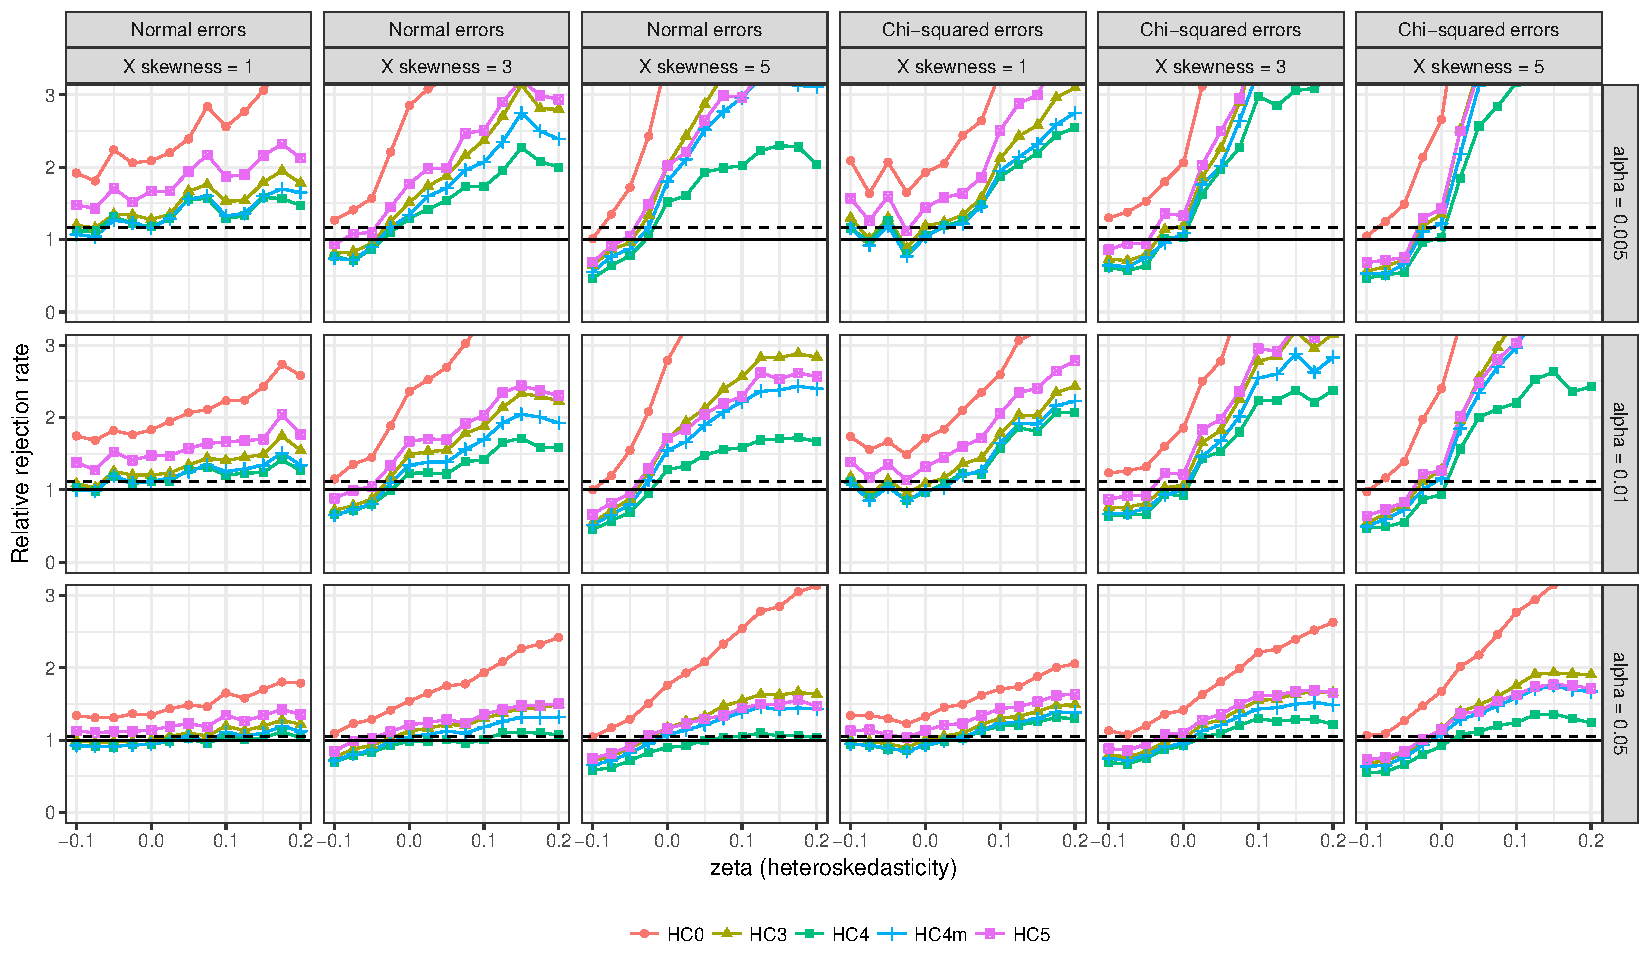
\includegraphics[width=\linewidth]{HC_fig/HC_size-1} 

}

\caption[Rejection rates of conventional tests based on HC3, HC4, HC4m, and HC5 for $n = 50$]{Rejection rates of conventional tests based on HC3, HC4, HC4m, and HC5 for $n = 50$. The solid horizontal line indicates the stated $\alpha$ level and the dashed line indicates an upper confidence bound on simulation error.}\label{fig:HC_size}
\end{figure}


\end{knitrout}

We first consider the empirical size of all seventeen tests. Figure \ref{fig:HC_size} depicts the rejection rates of the conventional t-tests based on the HC3, HC4, HC4m, and HC5 estimators, at a sample size of $n = 50$, as a function of the degree of heteroskedasticity. Each plot is repeated for varying degrees of skewness (columns) and nominal level (rows), and with either normal of $\chi^2_5$ errors (rows). Tests based on HC0, HC1, and HC2 have strictly higher rejection rates than HC3, and so we omit them from the figure. It can be seen that the test with HC3 does not maintain the nominal level except when the degree of heteroskedascity is small and skewness is mild. Its performance also degrades at smaller values of $\alpha$. The test with HC5 behaves similarly to that with HC3, but has even higher rejection rates when skewness is less severe. 

Of the conventional tests, using HC4 produces rejection rates that are closest to nominal across the conditions examined. At $\alpha = .05$, its rejection rates remain very close to nominal when errors are normal, although they are slightly larger than nominal when errors are $\chi^2_5$ and more strongly heteroskedastic. At lower values of $\alpha$, however, even HC4 has higher-than-nominal rejection rates, and these are more strongly affected by the degree of heteroskedasticity. Finally, rejection rates of the conventional test with HC4m are intermediate between those of HC4 and those of HC5. In further analysis, we focus only on the test with HC4 because its rejection rates are consistently closer to the nominal level across all conditions. 

\begin{knitrout}
\definecolor{shadecolor}{rgb}{0.969, 0.969, 0.969}\color{fgcolor}\begin{figure}[p]

{\centering 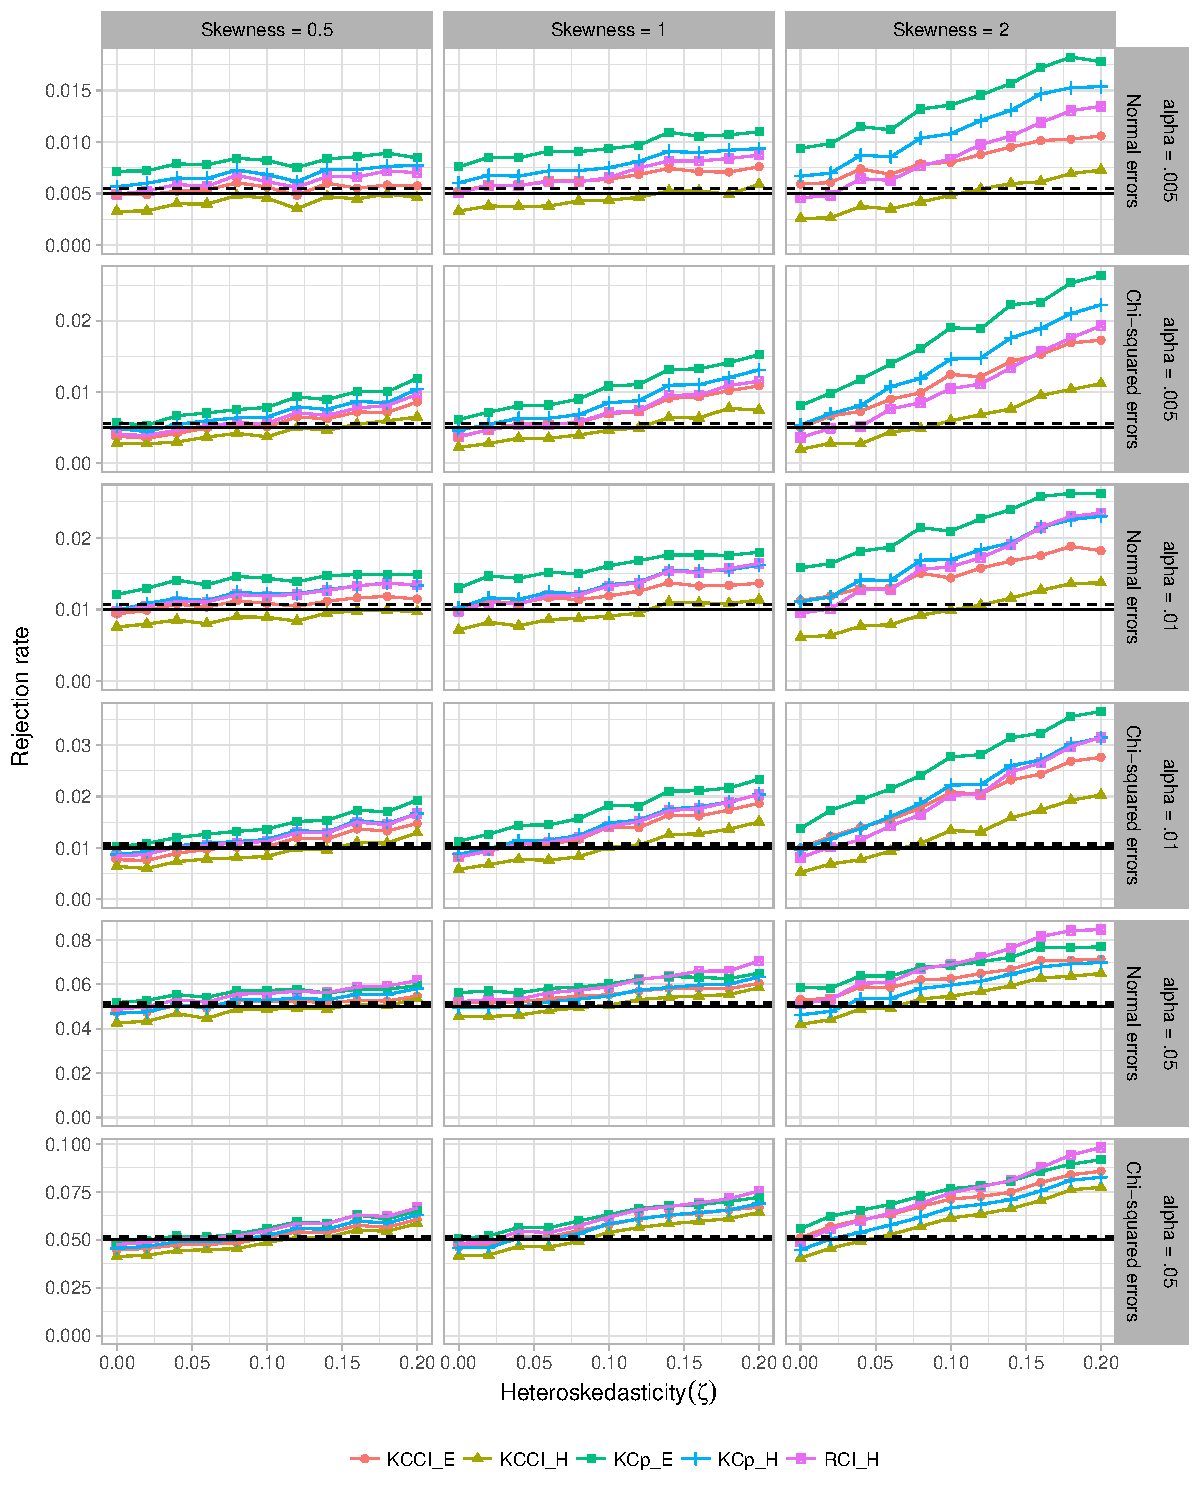
\includegraphics[width=\linewidth]{HC_fig/Edgeworth_size-1} 

}

\caption[Rejection rates of Edgeworth approximation tests for $n = 50$]{Rejection rates of Edgeworth approximation tests for $n = 50$. The solid horizontal line indicates the stated $\alpha$ level and the dashed line indicates an upper confidence bound on simulation error.}\label{fig:Edgeworth_size}
\end{figure}


\end{knitrout}

\begin{knitrout}
\definecolor{shadecolor}{rgb}{0.969, 0.969, 0.969}\color{fgcolor}\begin{figure}[p]

{\centering 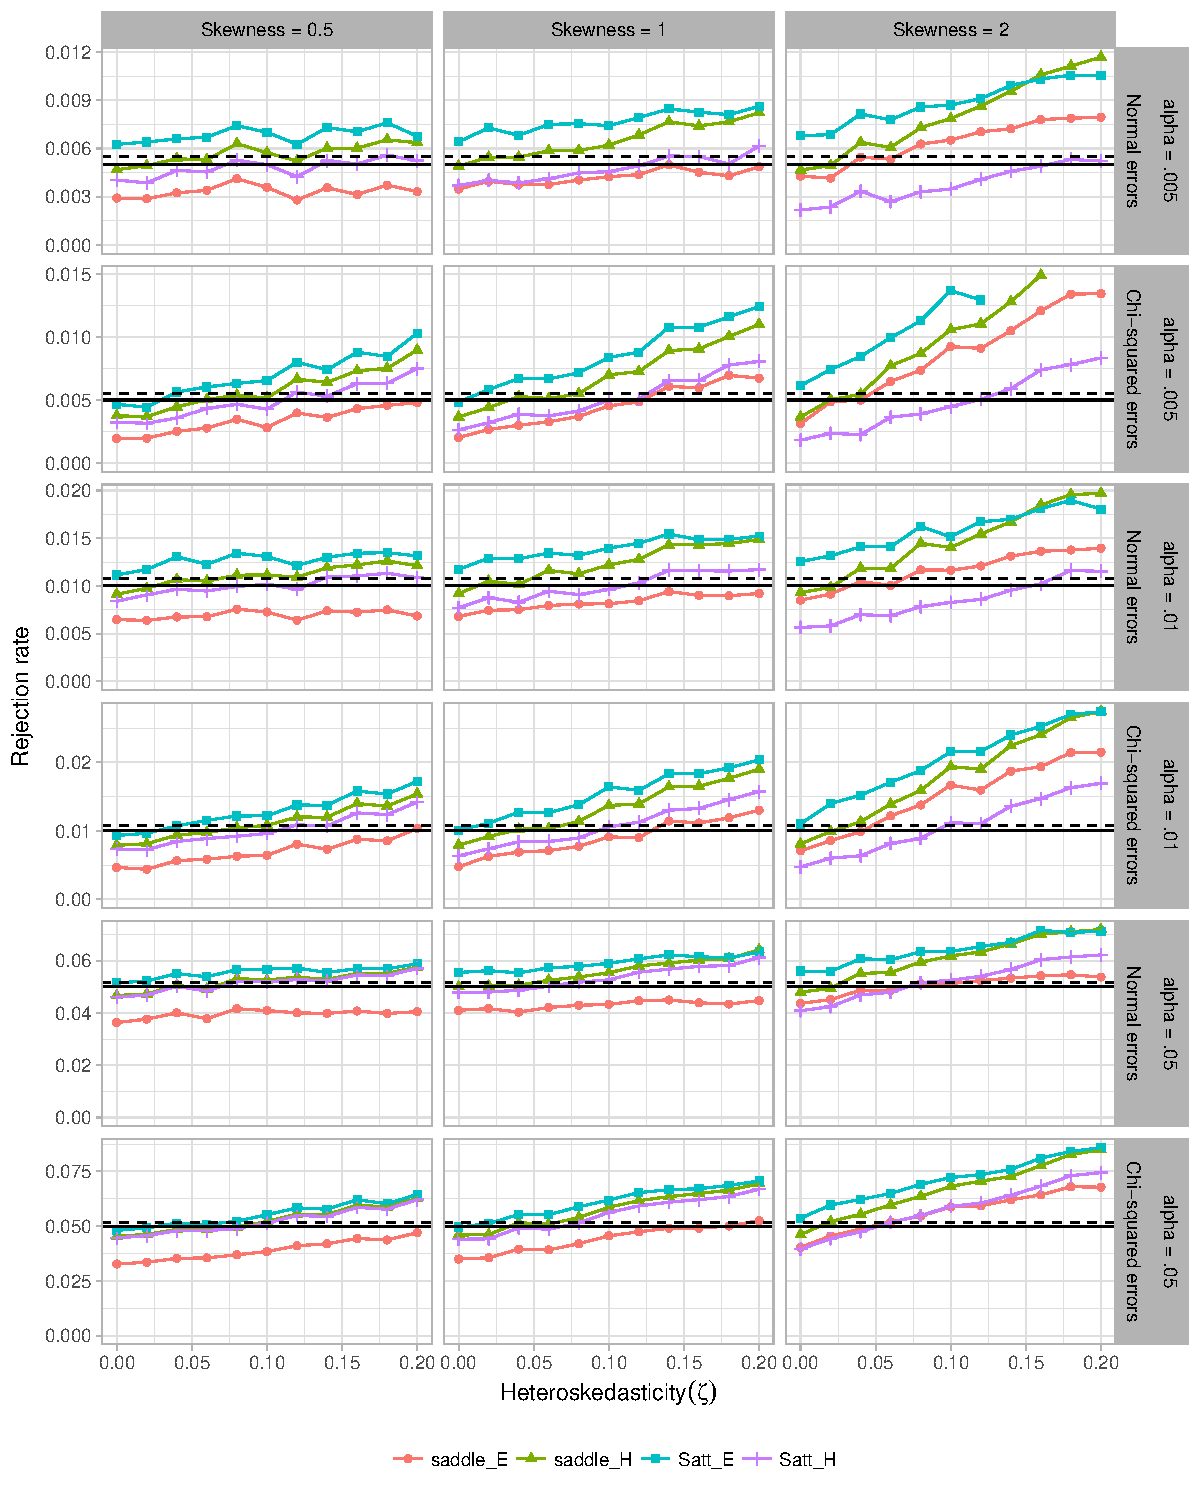
\includegraphics[width=\linewidth]{HC_fig/Satterthwaite_size-1} 

}

\caption[Rejection rates of Satterthwaite and saddlepoint approximation tests for $n = 50$]{Rejection rates of Satterthwaite and saddlepoint approximation tests for $n = 50$. The solid horizontal line indicates the stated $\alpha$ level and the dashed line indicates an upper confidence bound on simulation error.}\label{fig:Satterthwaite_size}
\end{figure}


\end{knitrout}

\begin{knitrout}
\definecolor{shadecolor}{rgb}{0.969, 0.969, 0.969}\color{fgcolor}\begin{figure}[p]

{\centering 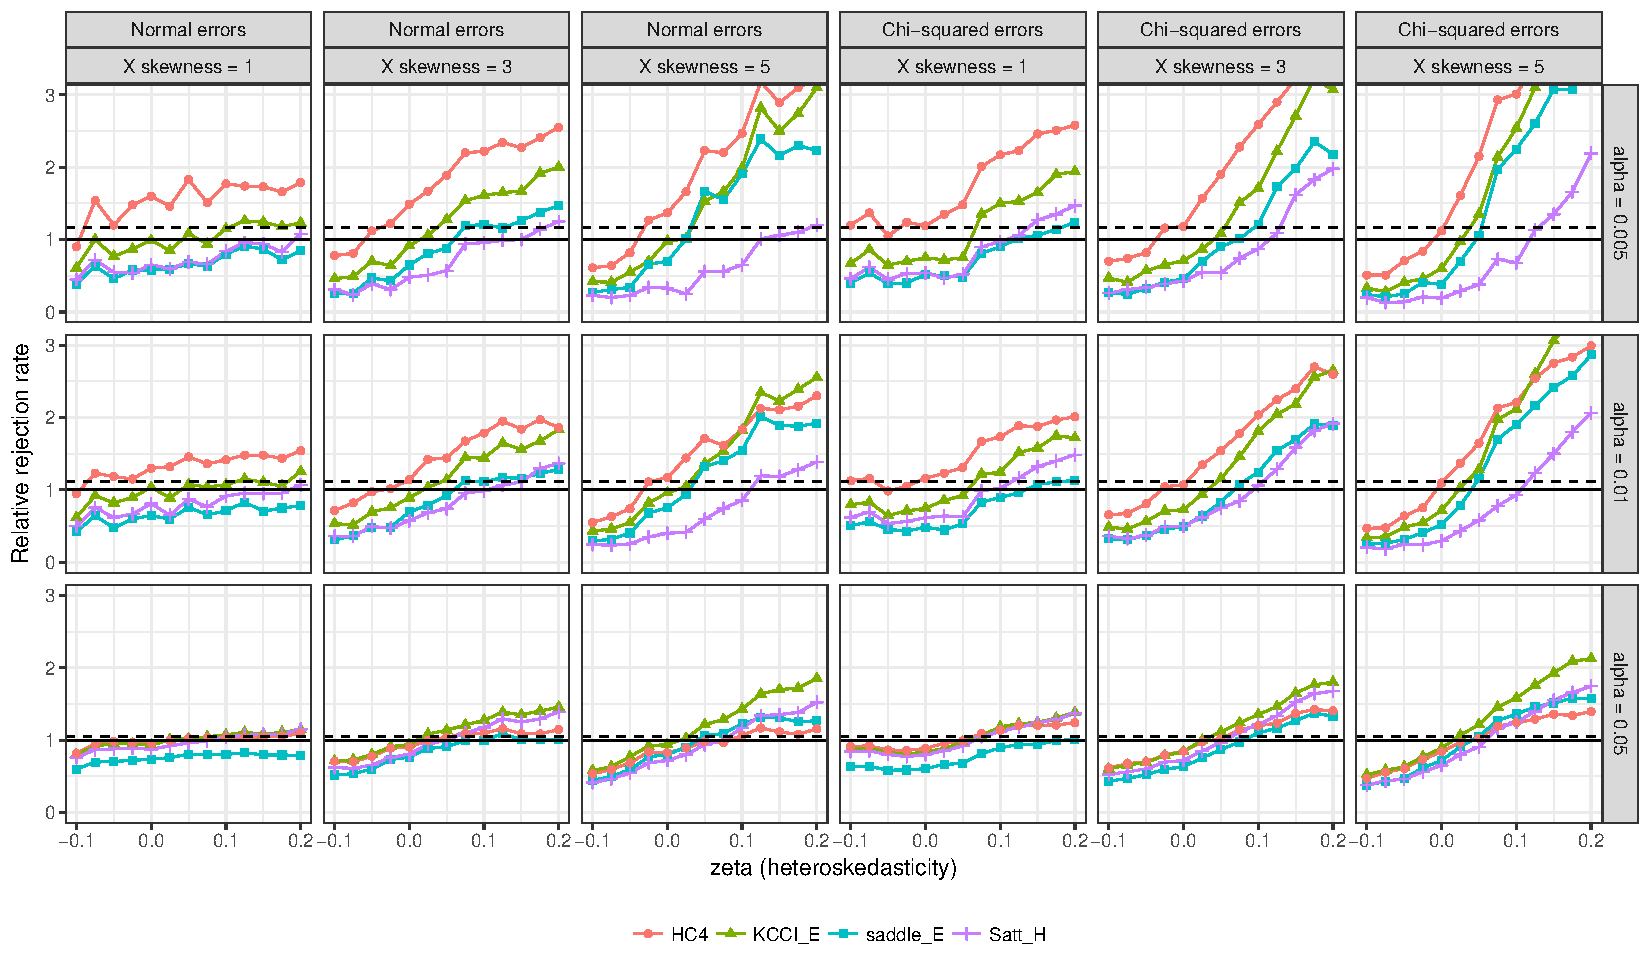
\includegraphics[width=\linewidth]{HC_fig/selected_size_25-1} 

}

\caption[Rejection rates of selected tests for $n = 25$]{Rejection rates of selected tests for $n = 25$. The solid horizontal line indicates the stated $\alpha$ level and the dashed line indicates an upper confidence bound on simulation error.}\label{fig:selected_size_25}
\end{figure}


\end{knitrout}

\begin{knitrout}
\definecolor{shadecolor}{rgb}{0.969, 0.969, 0.969}\color{fgcolor}\begin{figure}[p]

{\centering 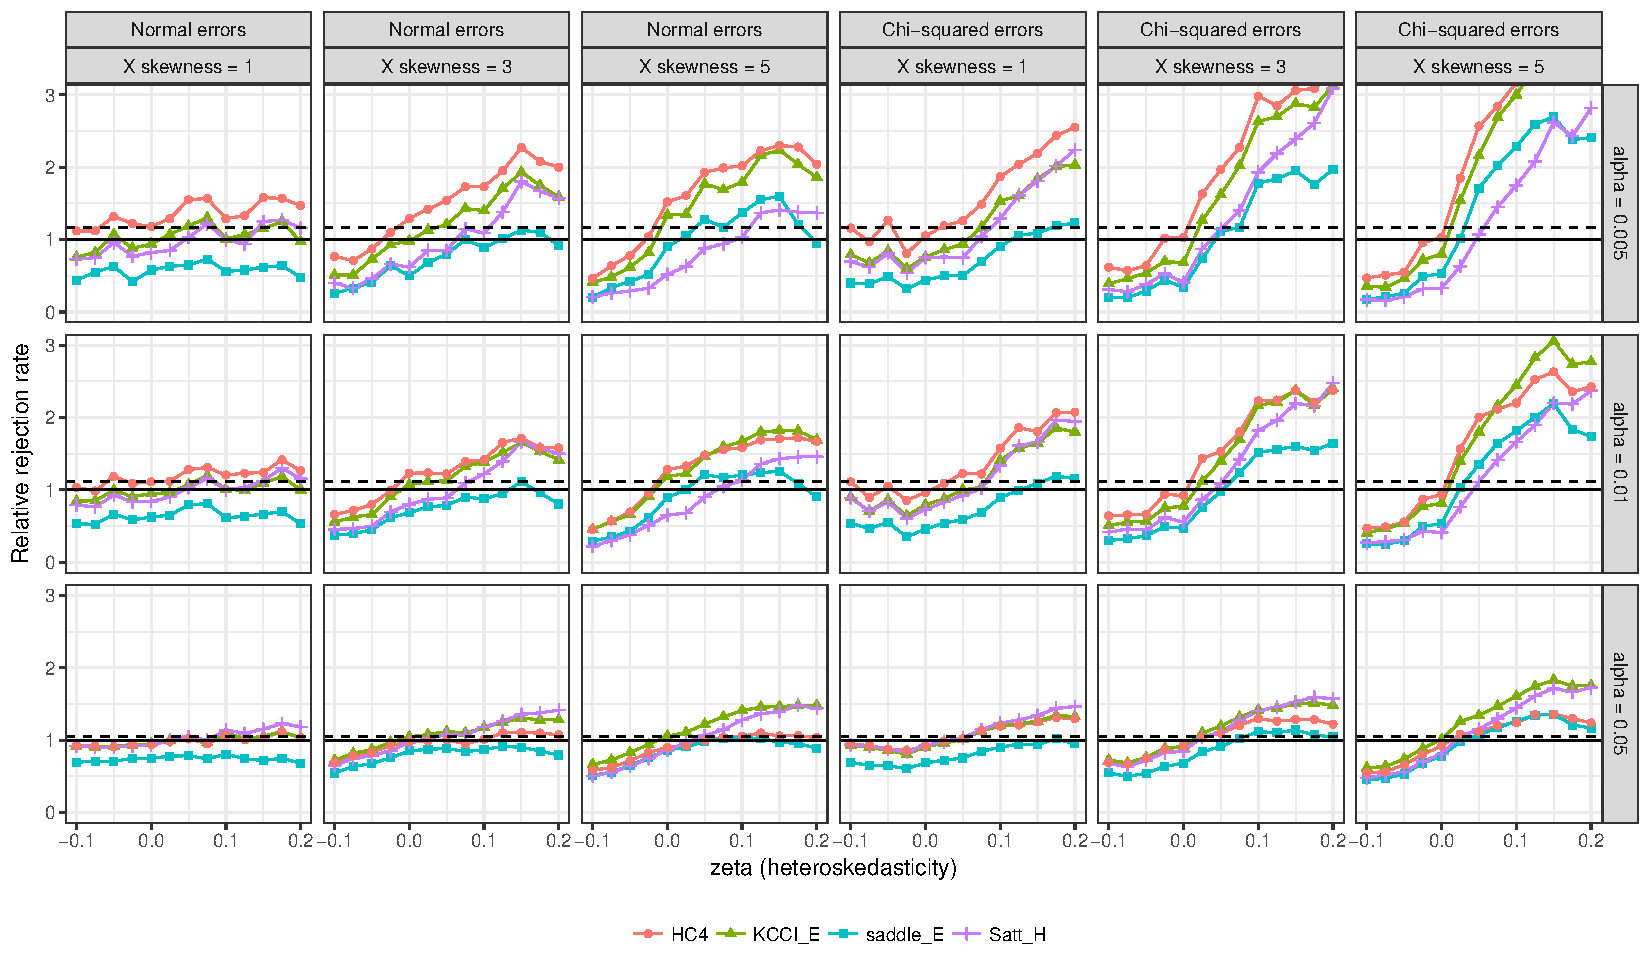
\includegraphics[width=\linewidth]{HC_fig/selected_size_50-1} 

}

\caption[Rejection rates of selected tests for $n = 50$]{Rejection rates of selected tests for $n = 50$. The solid horizontal line indicates the stated $\alpha$ level and the dashed line indicates an upper confidence bound on simulation error.}\label{fig:selected_size_50}
\end{figure}


\end{knitrout}

\begin{knitrout}
\definecolor{shadecolor}{rgb}{0.969, 0.969, 0.969}\color{fgcolor}\begin{figure}[p]

{\centering 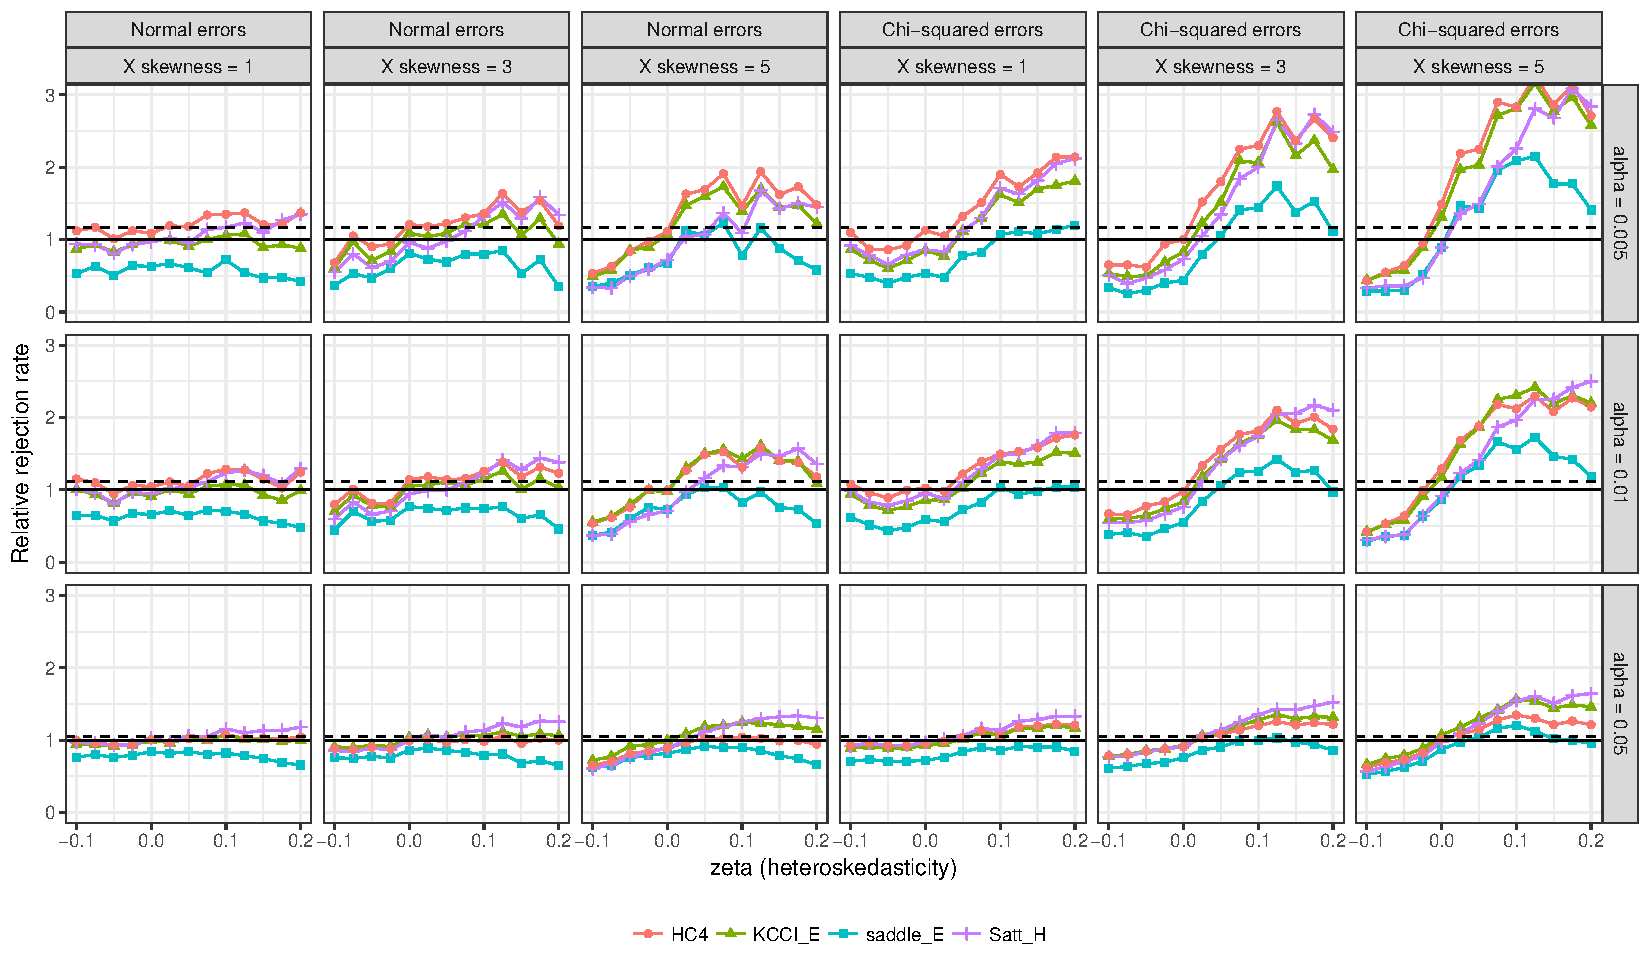
\includegraphics[width=\linewidth]{HC_fig/selected_size_100-1} 

}

\caption[Rejection rates of selected tests for $n = 100$]{Rejection rates of selected tests for $n = 100$. The solid horizontal line indicates the stated $\alpha$ level and the dashed line indicates an upper confidence bound on simulation error.}\label{fig:selected_size_100}
\end{figure}


\end{knitrout}

\section{Discussion}
\label{sec:conc}

Further research. 
Wild bootstrap tests.
Heteroskedasticity-robust F-tests Cite \citet{Cai2008new}.

\bibliographystyle{agsm}
\bibliography{Bibliography}

\end{document}
